\section{eo\-Real\-Vector\-No\-Bounds Class Reference}
\label{classeo_real_vector_no_bounds}\index{eoRealVectorNoBounds@{eoRealVectorNoBounds}}
the dummy unbounded {\bf eo\-Real\-Vector\-Bounds}{\rm (p.\,\pageref{classeo_real_vector_bounds})}: usefull if you don't need bounds! everything is inlined.  


{\tt \#include $<$eo\-Real\-Vector\-Bounds.h$>$}

Inheritance diagram for eo\-Real\-Vector\-No\-Bounds::\begin{figure}[H]
\begin{center}
\leavevmode
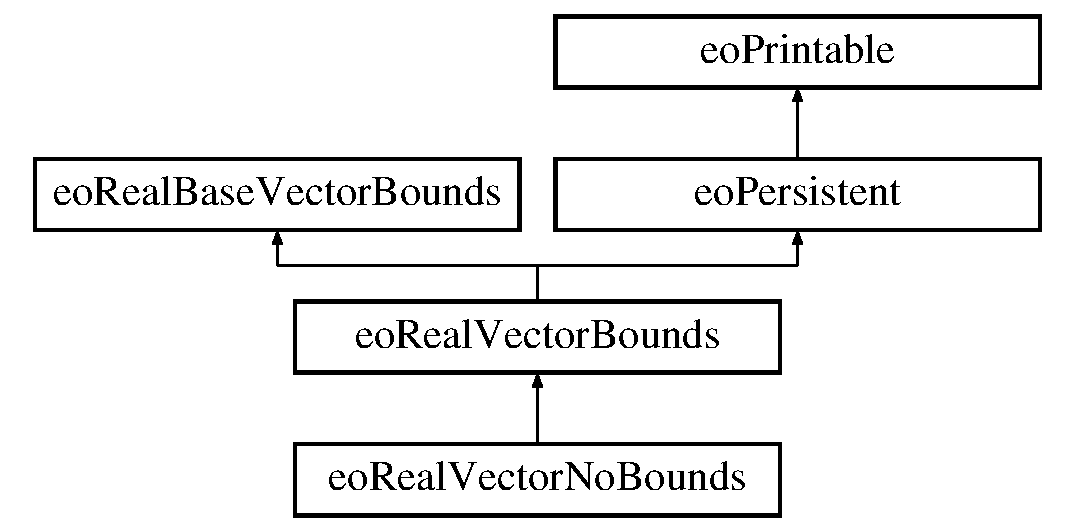
\includegraphics[height=4cm]{classeo_real_vector_no_bounds}
\end{center}
\end{figure}
\subsection*{Public Member Functions}
\begin{CompactItemize}
\item 
{\bf eo\-Real\-Vector\-No\-Bounds} (unsigned \_\-dim)\label{classeo_real_vector_no_bounds_a1}

\begin{CompactList}\small\item\em Ctor: nothing to do, but beware of dimension: call base class ctor. \item\end{CompactList}\item 
virtual bool {\bf is\-Bounded} (unsigned)\label{classeo_real_vector_no_bounds_a2}

\begin{CompactList}\small\item\em test: is i\_\-th component bounded \item\end{CompactList}\item 
virtual bool {\bf is\-Bounded} (void)\label{classeo_real_vector_no_bounds_a3}

\begin{CompactList}\small\item\em test: bounded iff all are bounded \item\end{CompactList}\item 
virtual bool {\bf has\-No\-Bound\-At\-All} (unsigned)\label{classeo_real_vector_no_bounds_a4}

\begin{CompactList}\small\item\em Self-test: true iff i\_\-th component has no bounds at all. \item\end{CompactList}\item 
virtual bool {\bf has\-No\-Bound\-At\-All} (void)\label{classeo_real_vector_no_bounds_a5}

\begin{CompactList}\small\item\em Self-test: true iff all components have no bound at all. \item\end{CompactList}\item 
virtual bool {\bf is\-Min\-Bounded} (unsigned)\label{classeo_real_vector_no_bounds_a6}

\item 
virtual bool {\bf is\-Max\-Bounded} (unsigned)\label{classeo_real_vector_no_bounds_a7}

\item 
virtual void {\bf folds\-In\-Bounds} (unsigned, double \&)\label{classeo_real_vector_no_bounds_a8}

\begin{CompactList}\small\item\em Folds a real value back into the bounds - i\_\-th component. \item\end{CompactList}\item 
virtual void {\bf folds\-In\-Bounds} (std::vector$<$ double $>$ \&)\label{classeo_real_vector_no_bounds_a9}

\begin{CompactList}\small\item\em Folds all variables of a std::vector of real values into the bounds. \item\end{CompactList}\item 
virtual void {\bf truncate} (unsigned, double \&)\label{classeo_real_vector_no_bounds_a10}

\begin{CompactList}\small\item\em Truncates a real value to the bounds - i\_\-th component. \item\end{CompactList}\item 
virtual void {\bf truncate} (std::vector$<$ double $>$ \&)\label{classeo_real_vector_no_bounds_a11}

\begin{CompactList}\small\item\em truncates all variables of a std::vector of real values to the bounds \item\end{CompactList}\item 
virtual bool {\bf is\-In\-Bounds} (unsigned, double)\label{classeo_real_vector_no_bounds_a12}

\begin{CompactList}\small\item\em test: is i\_\-th component within the bounds? \item\end{CompactList}\item 
virtual bool {\bf is\-In\-Bounds} (std::vector$<$ double $>$)\label{classeo_real_vector_no_bounds_a13}

\begin{CompactList}\small\item\em test: are ALL components within the bounds? \item\end{CompactList}\item 
virtual double {\bf minimum} (unsigned)\label{classeo_real_vector_no_bounds_a14}

\begin{CompactList}\small\item\em Accessors: will raise an std::exception if these do not exist. \item\end{CompactList}\item 
virtual double {\bf maximum} (unsigned)\label{classeo_real_vector_no_bounds_a15}

\item 
virtual double {\bf range} (unsigned)\label{classeo_real_vector_no_bounds_a16}

\item 
virtual double {\bf average\-Range} ()\label{classeo_real_vector_no_bounds_a17}

\begin{CompactList}\small\item\em Computes the average range An std::exception will be raised if one of the component is unbounded. \item\end{CompactList}\item 
virtual double {\bf uniform} (unsigned, {\bf eo\-Rng} \&\_\-rng=eo::rng)\label{classeo_real_vector_no_bounds_a18}

\begin{CompactList}\small\item\em Generates a random number in i\_\-th range An std::exception will be raised if one of the component is unbounded. \item\end{CompactList}\item 
void {\bf uniform} (std::vector$<$ double $>$ \&, {\bf eo\-Rng} \&\_\-rng=eo::rng)\label{classeo_real_vector_no_bounds_a19}

\begin{CompactList}\small\item\em fills a std::vector with uniformly chosen variables in bounds An std::exception will be raised if one of the component is unbounded \item\end{CompactList}\end{CompactItemize}


\subsection{Detailed Description}
the dummy unbounded {\bf eo\-Real\-Vector\-Bounds}{\rm (p.\,\pageref{classeo_real_vector_bounds})}: usefull if you don't need bounds! everything is inlined. 

Warning: we do need this class, and not only a std::vector$<$eo\-Real\-No\-Bounds $\ast$$>$ 



Definition at line 352 of file eo\-Real\-Vector\-Bounds.h.

The documentation for this class was generated from the following file:\begin{CompactItemize}
\item 
eo\-Real\-Vector\-Bounds.h\end{CompactItemize}
